\documentclass[12pt]{article}
% Преамбула

\usepackage[utf8]{inputenc}
\usepackage[T2A]{fontenc}
\usepackage[english,russian]{babel}
\usepackage{amssymb,amsmath}
\usepackage{multicol}
\usepackage{graphicx}
\usepackage{array,graphicx,caption}
\usepackage{hyperref}
\usepackage[procnames]{listings}
\usepackage{color}

\begin{document}
\thispagestyle{empty}
\begin{center}
\ \vspace{-3cm}
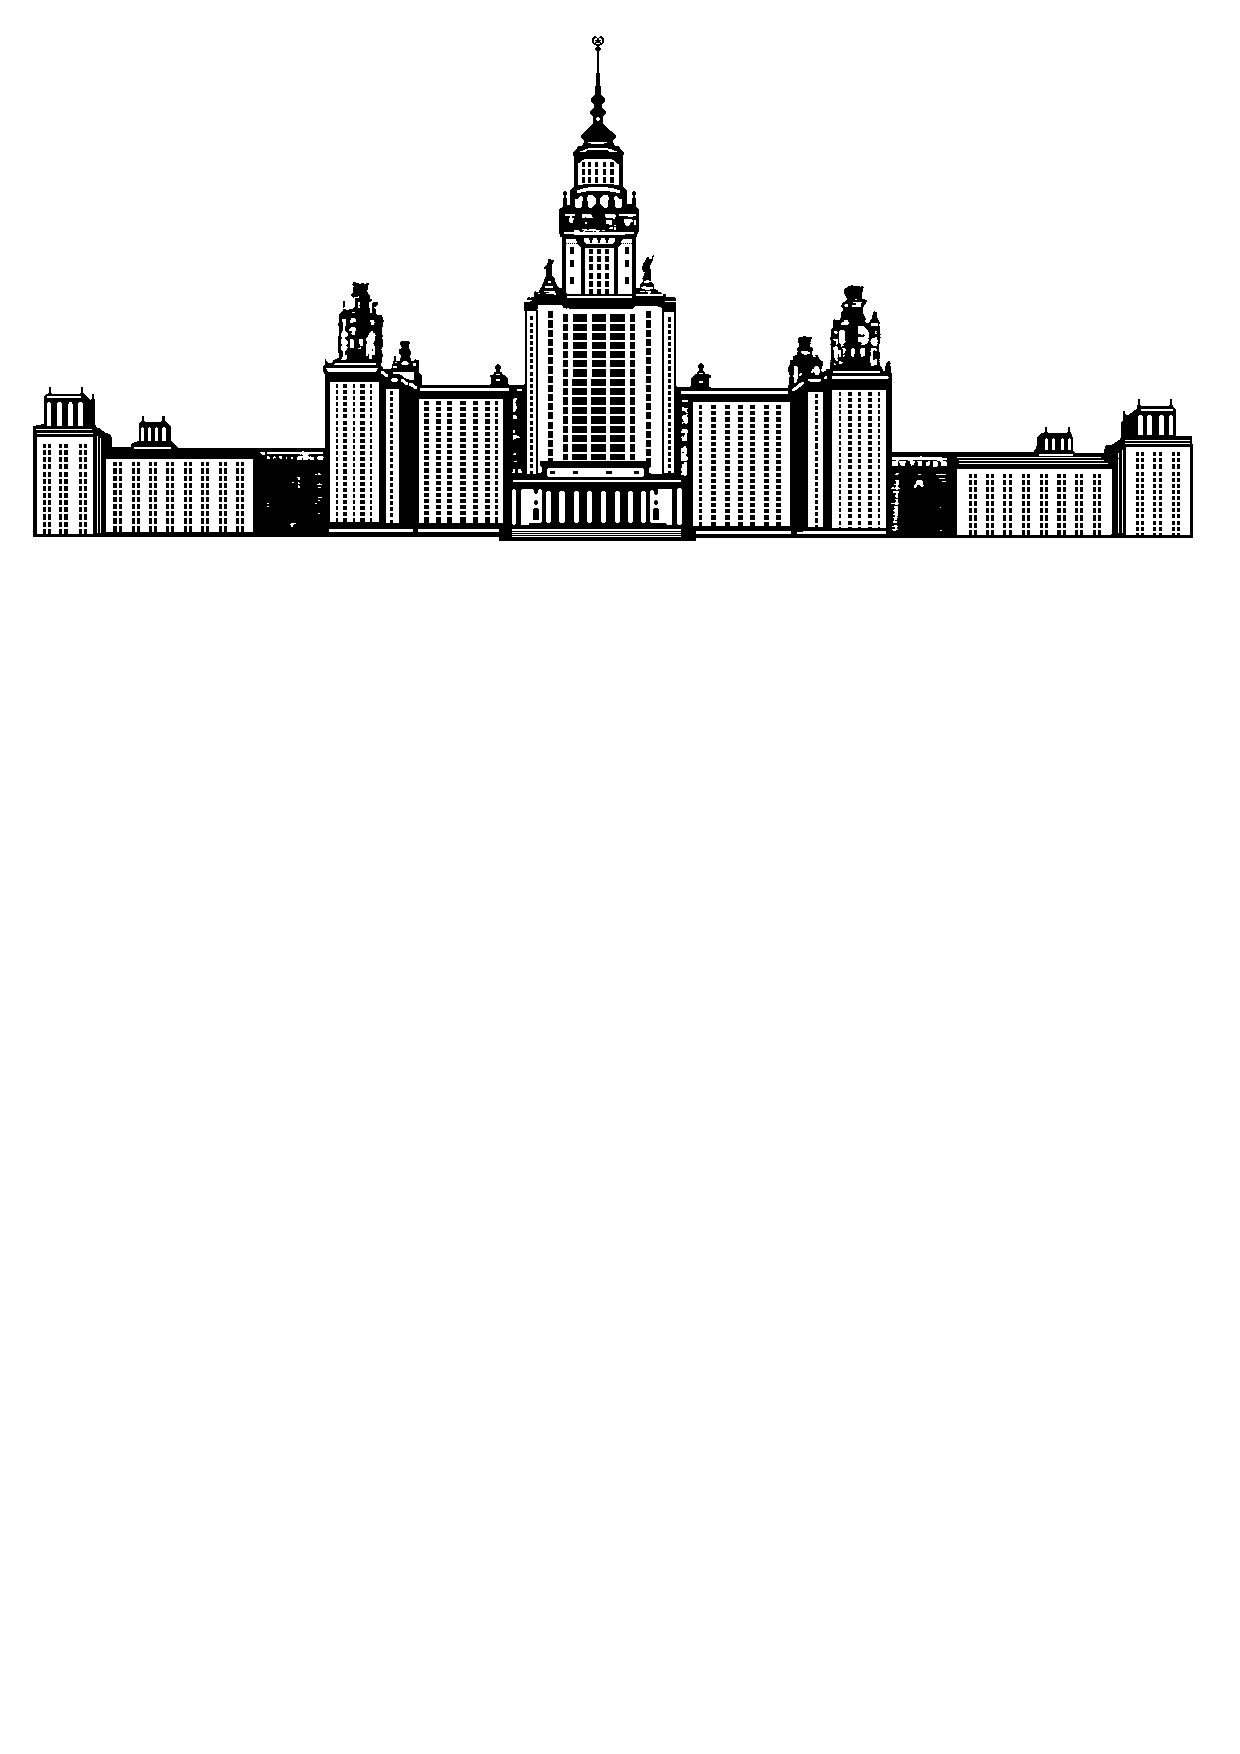
\includegraphics[width=0.3\textwidth]{i1.pdf}\\
{\scshape Московский государственный университет имени М.~В.~Ломоносова}\\
Факультет вычислительной математики и кибернетики\\
Кафедра системного анализа
\vfill
{\LARGE Отчёт по практикуму\\}
\vspace{1cm}
{\Huge\textbf\ <<Построение выпуклой оболочки>>}
\end{center}
\vspace{1cm}
\begin{flushright}
\large
\textit{Студентка 315 группы}\\
П.~Воронкова

\vspace{10mm}
\textit{Руководитель практикума}\\
А.~Месяц
\end{flushright}
\vfill
\begin{center}
Москва, 2015
\end{center}
\newpage
\section {Постановка задачи}
\indent Написать функцию, принимающую на вход два вектора координат, и возвращающую массив индексов точек, образующих выпуклую оболочку заданных точек. Выпуклая оболочка строится алгоритмом Киркпатрика.
\subsection{Основные определения}
\begin {itemize}
\item Выпуклой оболочкой множества $X$ называется наименьшее выпуклое множество, содержащее $X$.
\item Опорной функцией, или опорным функционалом, множества $M$, лежащего в векторном пространстве $V$, называется функция $s_M$, задаваемая на сопряжённом пространстве $V^*$ соотношением 
$$s_M (y) = \sup_{x\in M} y(x).$$
\item Опорной прямой к выпуклому многоугольнику  $P$  называется прямая  $l$, проходящая через некоторую вершину многоугольника  $P$  таким образом, что все внутренние точки многоугольника лежат по одну сторону от прямой  $l$ .
\end{itemize}
\section{Решение задачи}
При решении задачи было использовано два алгоритма ~--- Грэхэма и Киркпатрика. Сначала используется алгоритм Киркпатрика, при котором точки рекурсивно делятся на подмножества (до тех пор, пока мощность подмножества не превысит заранее заданного числа $N$). После этого выпуклая оболочка неделимого подмножества находится посредством аглоритма Грэхема. Затем находится выпуклая оболочка исходного множества как выпуклая оболочка объединения двух выпуклых многоугольников.
Рассмотрим алгоритмы подробнее.
\subsection {Алгоритм Киркпатрика.}
Построение выпуклой оболочки методом «разделяй и властвуй» ~--- алгоритм построения выпуклой оболочки.
Дано множество  S, состоящее из  N  точек.


Описание:
\begin {enumerate}
\item Если  $N \leqslant N_0$ ($N_0$ ~--- некоторое небольшое целое число), то построить выпуклую оболочку одним из известных методов и остановиться, иначе перейти к шагу 2.
\item Разобьем исходное множество  $S$  произвольным образом на два примерно равных по мощности подмножества $S_1$ и $S_2$ (пусть $S_1$ содержит  $N/2$  точек, а $S_2$ содержит  $N - N/2$  точек).
\item Рекурсивно находим выпуклые оболочки каждого из подмножеств $S_1$ и $S_2$.
\item Строим выпуклую оболочку исходного множества как выпуклую оболочку объединения двух выпуклых многоугольников  $CH(S_1)$  и  $CH(S_2)$ .
\end{enumerate}
\subsection {Алгоритм Грэхэма.}


Найдём самую левую и самую правую точки $A$ и $B$ (если таких точек несколько, то возьмём самую нижнюю среди левых, и самую верхнюю среди правых). Понятно, что и $A$, и $B$ обязательно попадут в выпуклую оболочку. Далее, проведём через них прямую $AB$, разделив множество всех точек на верхнее и нижнее подмножества $S_1$ и $S_2$ (точки, лежащие на прямой, можно отнести к любому множеству ~--- они всё равно не войдут в оболочку). Точки $A$ и $B$ отнесём к обоим множествам. 

Теперь построим для $S_1$ верхнюю оболочку, а для $S_2$ ~--- нижнюю оболочку, и объединим их, получив ответ. Чтобы получить, скажем, верхнюю оболочку, нужно отсортировать все точки по абсциссе, затем пройтись по всем точкам, рассматривая на каждом шаге кроме самой точки две предыдущие точки, вошедшие в оболочку. Если текущая тройка точек образует не правый поворот (что легко проверить с помощью Ориентированной площади), то ближайшего соседа нужно удалить из оболочки. В конце концов, останутся только точки, входящие в выпуклую оболочку.

\subsection {Выпуклая оболочка объединения двух выпуклых многоугольников.}
Пусть мы уже имеем построенные выпуклые оболочки  $P_1$  и  $P_2$ .
Найдём некоторую внутреннюю точку  $A$  многоугольника  $P_1$  (например, центроид любых трёх вершин  $P_1$). Такая точка  $A$  будет внутренней точкой  $CH(P_1 \cup P_2)$.
Возможны два случая:
\begin{enumerate}
\item Точка  $A$  не является внутренней точкой многоугольника  $P_2$.\\
Проводим две опорные прямые для многоугольника  $P_2$, проходящие через точку  $A$. Эти опорные прямые проходят через вершины  B  и  C  многоугольника  $P_2$. Все точки внутри треугольника  $ABC$  не принадлежат границе выпуклой оболочки  $CH(P1 \cup P2)$. Все остальные точки упорядочиваем по полярному углу относительно точки  $A$, слиянием двух упорядоченных списков вершин за время  $O(N_1) + O(N_2) = O(N)$, а затем применяем к полученному списку метод обхода Грэхема, требующий лишь линейное время.
\item Точка  $A$  является внутренней точкой многоугольника  $P_2$. \\
Упорядочиваем вершины обоих многоугольников относительно центра  $A$, сливая два упорядоченных списка вершин  $P_1$  и  $P_2$  за  $O(N)$.
Теперь к полученному списку вершин можно применить алгоритм Грэхема за исключением фазы сортировки точек по полярной координате, тогда он будет выполнен за линейное время.
Теперь получена выпуклая оболочка объединения выпуклых многоугольников  $P_1 \cup P_2$.
\end{enumerate}
\section {Примеры работы алгоритма}
Примеры работы программы изображены на рисунках ~\ref{fig:1} -- ~\ref{fig:4}. Сравнение времени работы программы и встроенной функции Matlab convexhull изображено на рис. ~\ref{fig:5}.

\begin {figure}[ht]
	\centering
   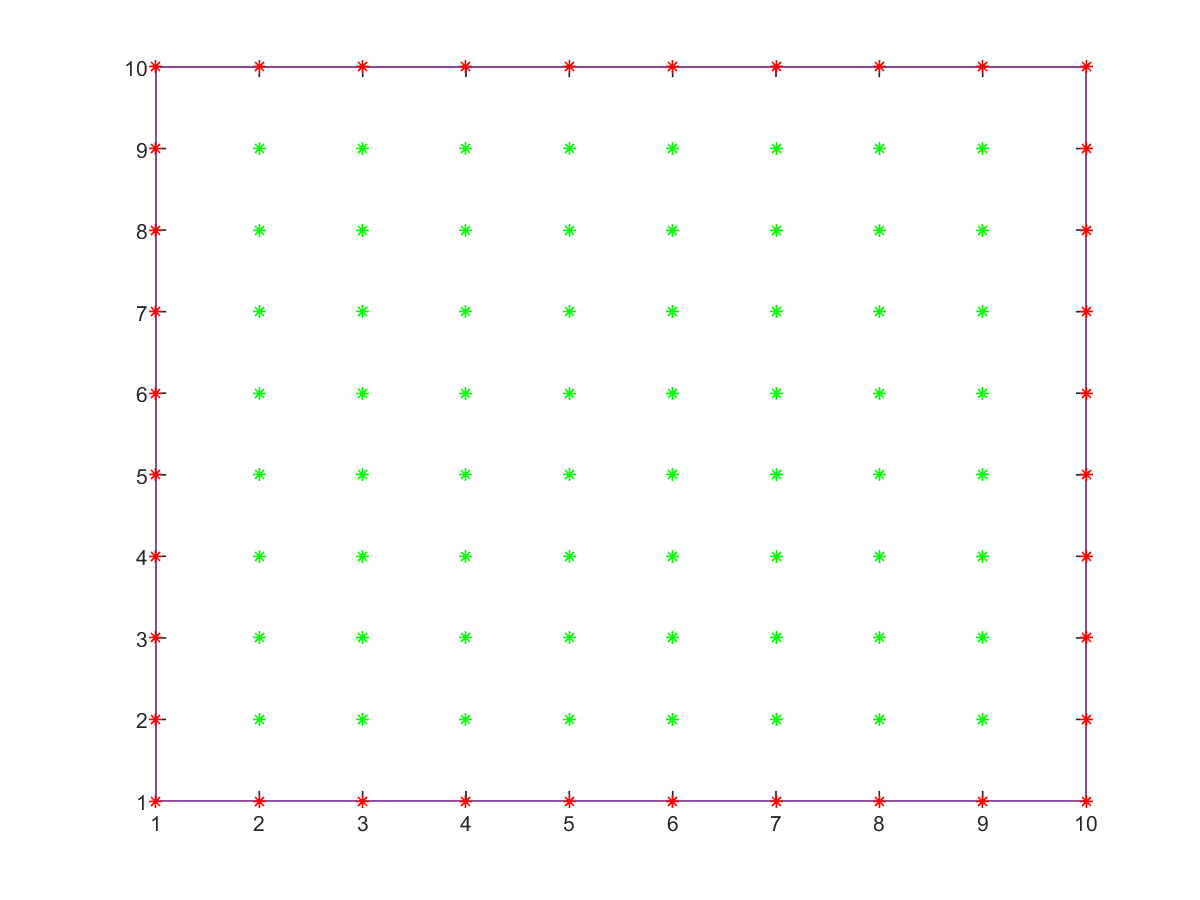
\includegraphics[width=0.7\textwidth]{1.png}
   \caption{100 элементов с равномерным распределением по всему координатному прямоугольнику. Время работы 1.26 с.}
		\label{fig:1}
\end{figure}
\begin {figure}[ht]
\centering
   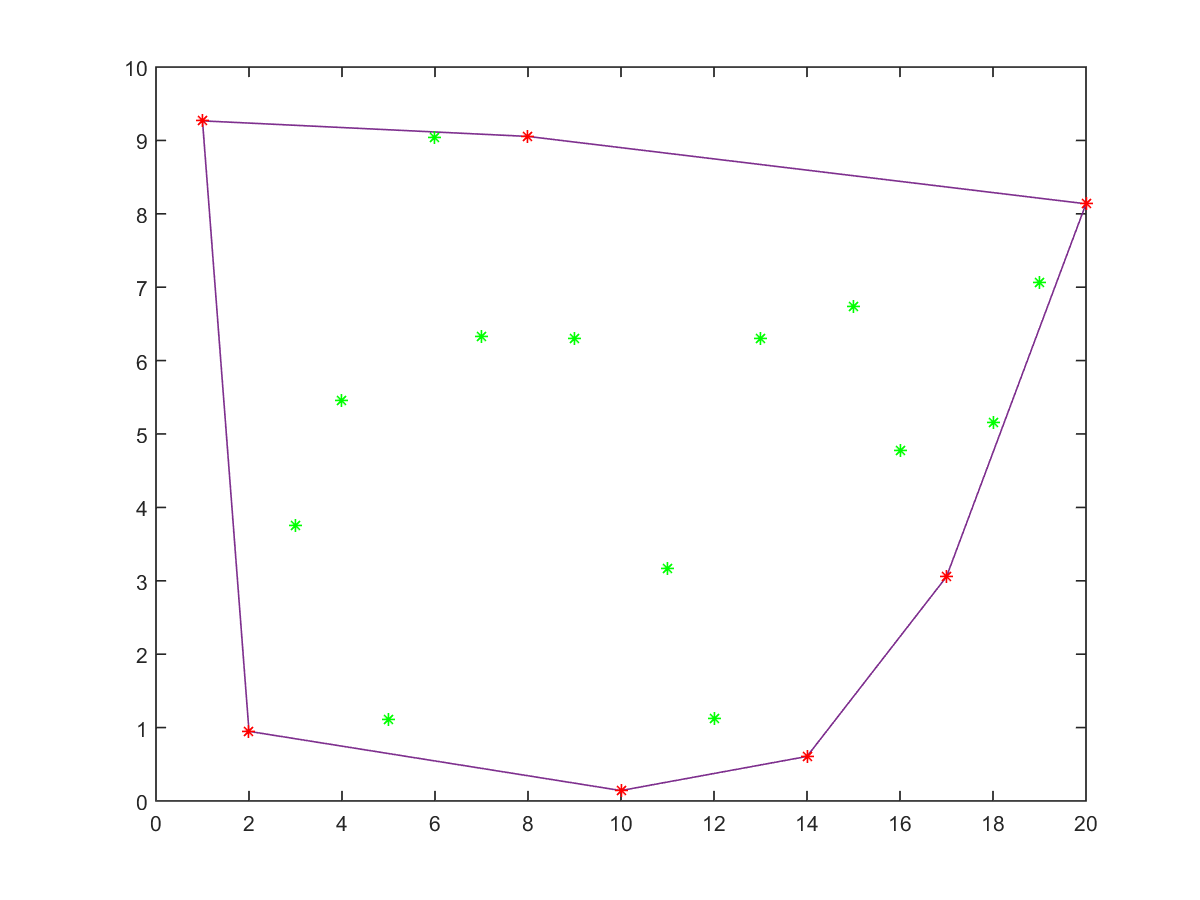
\includegraphics[width=0.7\textwidth]{2.png}
   \caption{20 элементов с равномерным распределением. Время работы программы 0.96 c.}
\end{figure}
\begin {figure}[ht]
\centering
   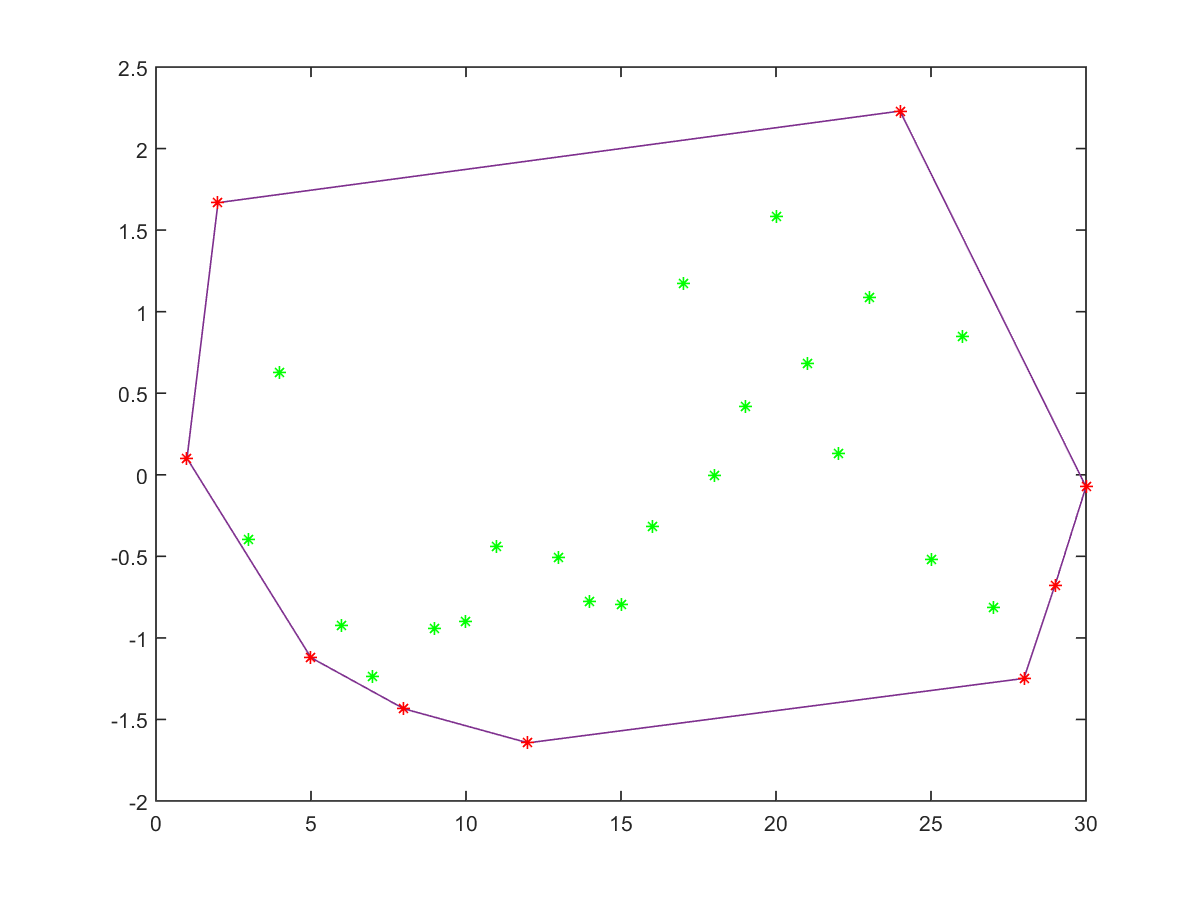
\includegraphics[width=0.7\textwidth]{3.png}
   \caption{Третий набор данных: 30 элементов с нормальным распределением. Время работы программы 0.88 c.}
\end{figure}
\begin {figure}[ht]
\centering
   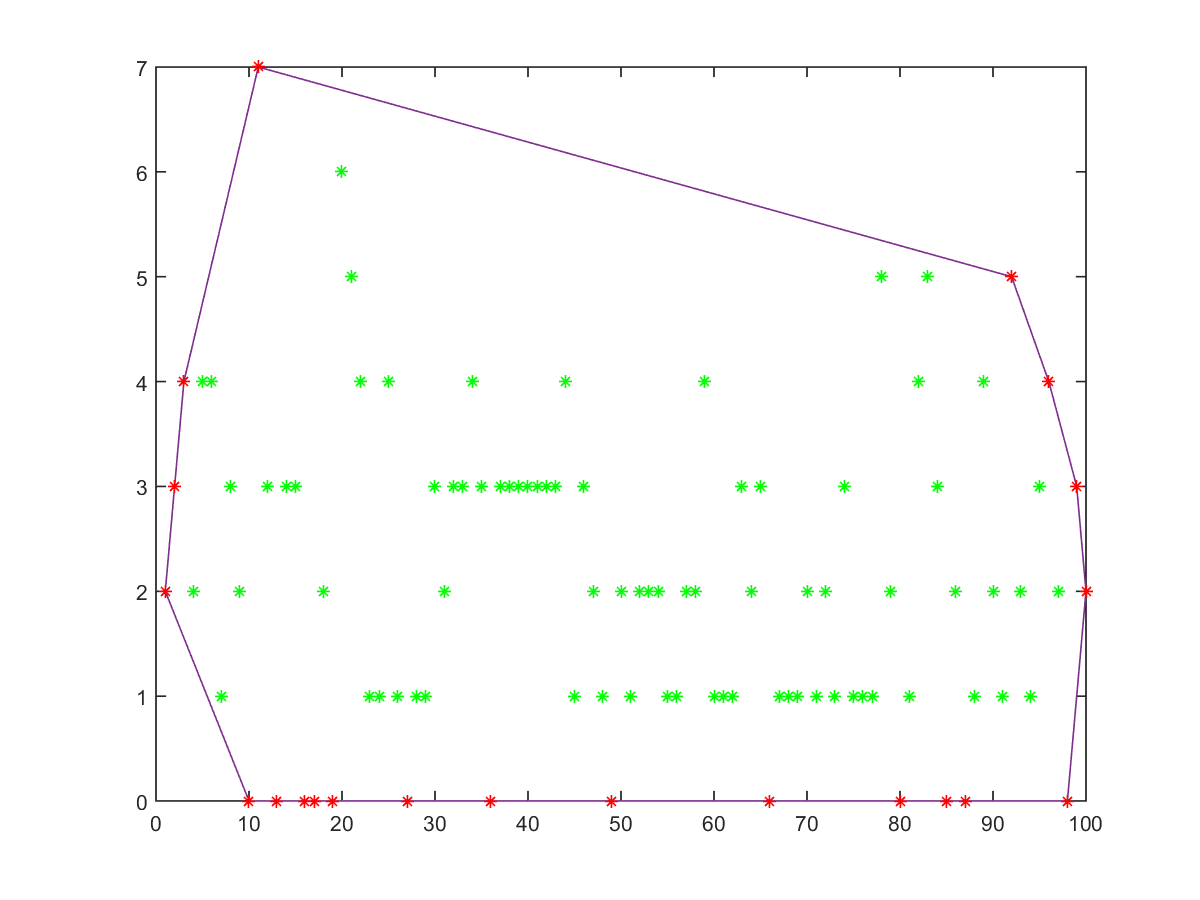
\includegraphics[width=0.7\textwidth]{4.png}
   \caption{Четвертый  набор данных: 100 элементов с пуассоновским распределением. Время работы программы 1.03 c.}
			\label{fig:4}
\end{figure}
\begin {figure}[ht]
\centering
   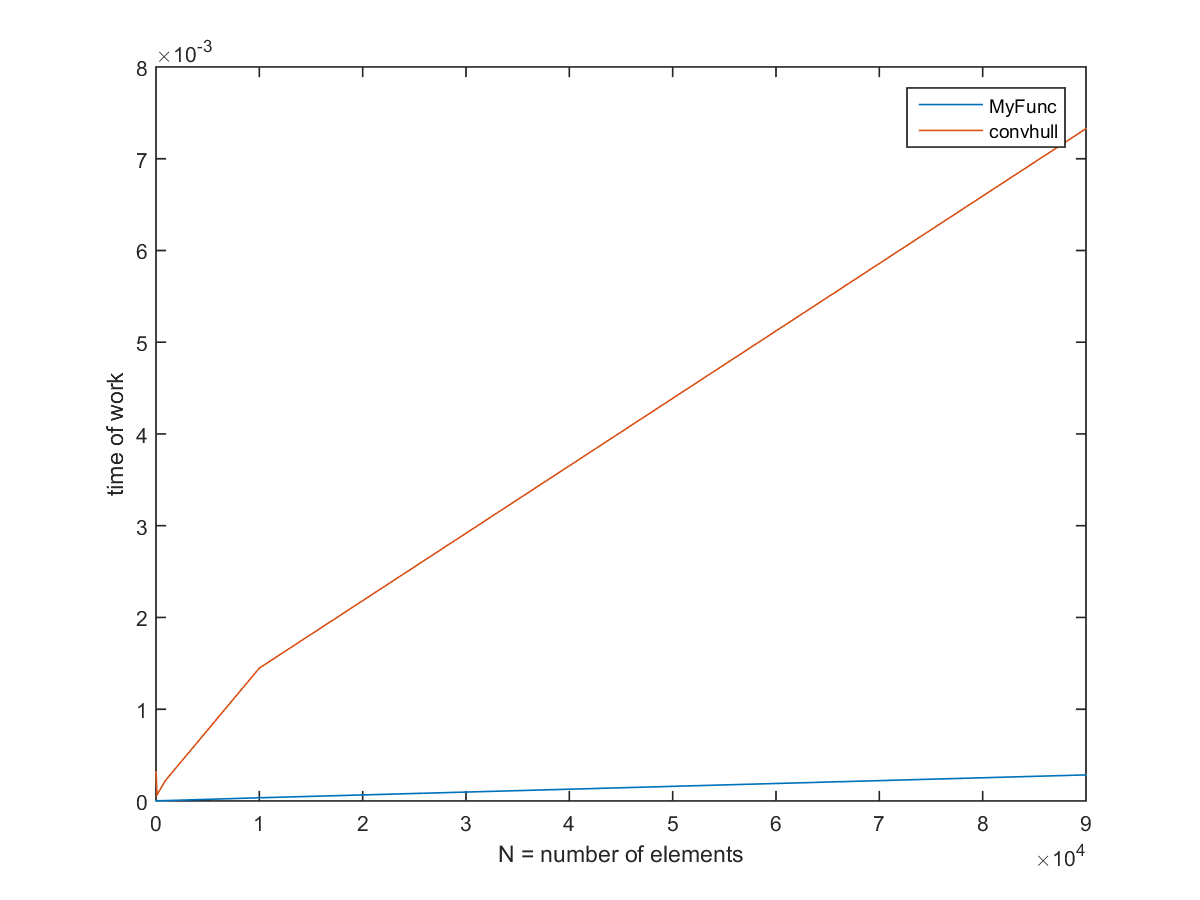
\includegraphics[width=0.9\textwidth]{g1.png}
   \caption{График сравнения времени работы}
				\label{fig:5}
\end{figure}
\end{document}
